\phantomsection
\section*{Chapter 7}
\addcontentsline{toc}{section}{Chapter 7}

\subsection*{7.1}

\begin{figure}[H]
  \centering
  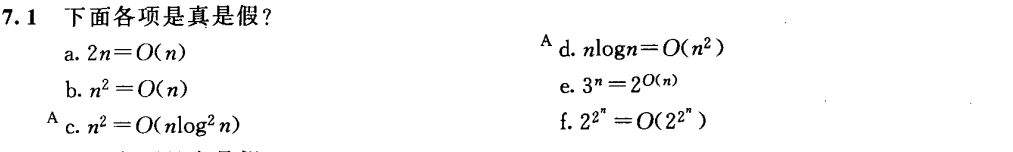
\includegraphics[width=\textwidth]{chapters/imgs/hw_7_1.png}
  \caption{}
  \label{fig:hw_7_1}
\end{figure}

\subsubsection*{解答}
 
\paragraph{(a) $2n = O(n)$ —— \textbf{真}.}
取常数 $c = 2$,$n_0 = 1$。对所有 $n \geq n_0$,有
\[
    2n \leq 2 \cdot n = c \cdot n,
\]
因此 $2n = O(n)$。
 
\paragraph{(b) $n^2 = O(n)$ —— \textbf{假}.}
假设存在常数 $c > 0$ 和 $n_0$ 使得对所有 $n \geq n_0$ 有 $n^2 \leq c n$。
两边同除以 $n$(此处 $n > 0$),得
\[
    n \leq c,
\]
但 $n$ 可以任意大,这与 $c$ 为固定常数矛盾。故 $n^2 \neq O(n)$。
 
\paragraph{(c) $n^2 = O(n \log^2 n)$ —— \textbf{假}.}
考察极限
\[
    \lim_{n \to \infty} \frac{n^2}{n \log^2 n}
    \;=\; \lim_{n \to \infty} \frac{n}{\log^2 n}
    \;=\; +\infty.
\]
比值趋于无穷,说明不存在常数 $c$ 使得 $n^2 \leq c \cdot n \log^2 n$ 对足够大的 $n$ 恒成立。故 $n^2 \neq O(n \log^2 n)$。
 
\paragraph{(d) $n \log n = O(n^2)$ —— \textbf{真}.}
对所有 $n \geq 1$,有 $\log n \leq n$,因此
\[
    n \log n \;\leq\; n \cdot n \;=\; n^2.
\]
取 $c = 1$,$n_0 = 1$ 即可。故 $n \log n = O(n^2)$。
 
\paragraph{(e) $3^n = 2^{O(n)}$ —— \textbf{真}.}
利用换底公式
\[
    3^n \;=\; \left(2^{\log_2 3}\right)^n \;=\; 2^{\,n \log_2 3}.
\]
由于 $\log_2 3 \approx 1.585$ 是常数,故 $n \log_2 3 = O(n)$,即存在常数 $c = \log_2 3$ 使得
$n \log_2 3 \leq c n$。因此 $3^n = 2^{O(n)}$。
 
\paragraph{(f) $2^{2^n} = O(2^{2^n})$ —— \textbf{真}.}
任何函数 $f(n)$ 都满足 $f(n) = O(f(n))$:取 $c = 1$,$n_0 = 1$,显然
\[
    2^{2^n} \;\leq\; 1 \cdot 2^{2^n}.
\]
故 $2^{2^n} = O(2^{2^n})$。
 
\paragraph{案：} 结合Big-O和Small-O记号的定义，可无惑。

\subsection*{7.2}

\begin{figure}[H]
  \centering
  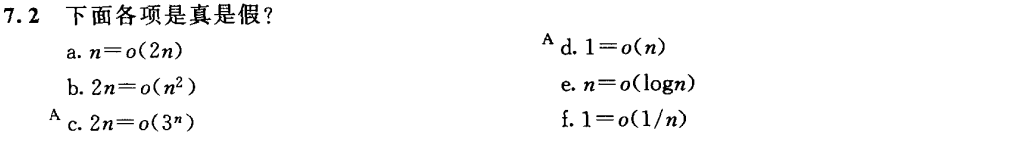
\includegraphics[width=\textwidth]{chapters/imgs/hw_7_2.png}
  \caption{}
  \label{fig:hw_7_2}
\end{figure}

\paragraph{小 $o$ 的定义回顾.}
$f(n) = o\bigl(g(n)\bigr)$ 当且仅当
\[
    \lim_{n \to \infty} \frac{f(n)}{g(n)} = 0.
\]
也就是说,$f$ 相对于 $g$ 是“真正可忽略”的;仅仅相差常数倍并不满足小 $o$ 关系。
 
\subsubsection*{解答}
 
\paragraph{(a) $n = o(2n)$ —— \textbf{假}.}
\[
    \lim_{n \to \infty} \frac{n}{2n} \;=\; \frac{1}{2} \;\neq\; 0.
\]
$n$ 与 $2n$ 只相差常数因子,属于同阶,不满足小 $o$ 关系。
 
\paragraph{(b) $2n = o(n^2)$ —— \textbf{真}.}
\[
    \lim_{n \to \infty} \frac{2n}{n^2} \;=\; \lim_{n \to \infty} \frac{2}{n} \;=\; 0.
\]
故 $2n = o(n^2)$。
 
\paragraph{(c) $2^n = o(3^n)$ —— \textbf{真}.}
\[
    \lim_{n \to \infty} \frac{2^n}{3^n}
    \;=\; \lim_{n \to \infty} \left(\frac{2}{3}\right)^n
    \;=\; 0,
\]
因为底数 $2/3 < 1$。故 $2^n = o(3^n)$。
 
\paragraph{(d) $1 = o(n)$ —— \textbf{真}.}
\[
    \lim_{n \to \infty} \frac{1}{n} \;=\; 0.
\]
故 $1 = o(n)$。
 
\paragraph{(e) $n = o(\log n)$ —— \textbf{假}.}
由洛必达法则(或基本增长速度比较)
\[
    \lim_{n \to \infty} \frac{n}{\log n} \;=\; +\infty.
\]
比值发散而非趋于 $0$,故 $n \neq o(\log n)$。
事实上关系恰好相反:$\log n = o(n)$。
 
\paragraph{(f) $1 = o(1/n)$ —— \textbf{假}.}
\[
    \lim_{n \to \infty} \frac{1}{\,1/n\,} \;=\; \lim_{n \to \infty} n \;=\; +\infty.
\]
比值发散,故 $1 \neq o(1/n)$。
正确的关系是 $1/n = o(1)$。
 
\paragraph{案：} 结合Big-O和Small-O记号的定义，可无惑。

\subsection*{7.5}

\begin{figure}[H]
  \centering
  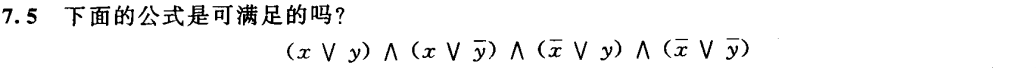
\includegraphics[width=\textwidth]{chapters/imgs/hw_7_5.png}
  \caption{}
  \label{fig:hw_7_5}
\end{figure}

\subsubsection*{解答}
 
\paragraph{枚举验证.}
只有两个变量 $x, y$,共有 $2^2 = 4$ 种真值赋值。
下表枚举全部可能:
 
\begin{center}
\renewcommand{\arraystretch}{1.25}
\begin{tabular}{|c|c||c|c|c|c||c|}
\hline
$x$ & $y$ & $x \vee y$ & $x \vee \bar{y}$ & $\bar{x} \vee y$ & $\bar{x} \vee \bar{y}$ & $\varphi$ \\
\hline\hline
0 & 0 & \textbf{0} & 1 & 1 & 1 & \textbf{0} \\
\hline
0 & 1 & 1 & \textbf{0} & 1 & 1 & \textbf{0} \\
\hline
1 & 0 & 1 & 1 & \textbf{0} & 1 & \textbf{0} \\
\hline
1 & 1 & 1 & 1 & 1 & \textbf{0} & \textbf{0} \\
\hline
\end{tabular}
\end{center}
 
\noindent 对于每一组赋值,总能找到至少一个子句的取值为 $0$,于是整个合取式为 $0$。
 
\paragraph{结构化解释.}
两变量的二元析取子句一共恰好有 $4$ 个,而每个子句 $(\ell_1 \vee \ell_2)$ 只在令 $\ell_1, \ell_2$ 同时为假时取 $0$,即恰好排除 $\{0,1\}^2$ 中的一个赋值:
\[
    \begin{array}{l@{\;:\;}l}
        (x \vee y)                 & \text{排除 } (x,y)=(0,0), \\
        (x \vee \bar{y})           & \text{排除 } (x,y)=(0,1), \\
        (\bar{x} \vee y)           & \text{排除 } (x,y)=(1,0), \\
        (\bar{x} \vee \bar{y})     & \text{排除 } (x,y)=(1,1).
    \end{array}
\]
这四个子句合取起来,恰把 $\{0,1\}^2$ 的全部四种赋值全部排除,因此没有任何赋值能令公式为真。
 
\paragraph{结论.}
\[
    \varphi \,\equiv\, \mathbf{0},
\]
即 $\varphi$ 是一个矛盾式,\textbf{不可满足}(unsatisfiable)。
 

\subsection*{7.7}

\begin{figure}[H]
  \centering
  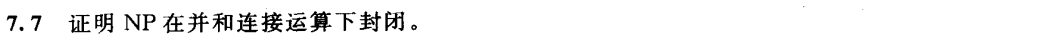
\includegraphics[width=\textwidth]{chapters/imgs/hw_7_7.png}
  \caption{}
  \label{fig:hw_7_7}
\end{figure}

 
即:若 $A, B \in \mathbf{NP}$,则 $A \cup B \in \mathbf{NP}$ 且 $A \circ B \in \mathbf{NP}$。
 
\paragraph{总体思路.}
由 $A, B \in \mathbf{NP}$,存在非确定型图灵机 $N_A$ 和 $N_B$,分别在多项式时间内判定 $A$ 和 $B$。
设 $N_A$ 的运行时间为 $O(n^{k_1})$,$N_B$ 的运行时间为 $O(n^{k_2})$,其中 $k_1, k_2$ 为常数。
我们分别构造两个非确定型图灵机 $N_\cup$ 与 $N_\circ$ 判定 $A \cup B$ 与 $A \circ B$。
 
\subsubsection*{第一部分:并封闭}
 
\paragraph{构造 $N_\cup$.} 对输入 $w$:
\begin{enumerate}
    \item 非确定地在以下两个分支中选择其一:
    \begin{itemize}
        \item \textbf{分支 1}:在 $w$ 上模拟 $N_A$;若 $N_A$ 接受则接受,否则拒绝。
        \item \textbf{分支 2}:在 $w$ 上模拟 $N_B$;若 $N_B$ 接受则接受,否则拒绝。
    \end{itemize}
\end{enumerate}
 
\paragraph{正确性.}
\[
    w \in A \cup B 
    \;\Longleftrightarrow\; w \in A \text{ 或 } w \in B 
    \;\Longleftrightarrow\; N_A \text{ 接受 } w \text{ 或 } N_B \text{ 接受 } w.
\]
而 $N_\cup$ 接受 $w$ 当且仅当其某个非确定分支接受 $w$,因此 $N_\cup$ 恰好判定 $A \cup B$。
 
\paragraph{时间分析.}
每个分支的运行时间为 $O(n^{k_1})$ 或 $O(n^{k_2})$,因此 $N_\cup$ 的运行时间为 $O(n^{\max(k_1, k_2)})$,
仍为多项式。故 $A \cup B \in \mathbf{NP}$。
 
\subsubsection*{第二部分:连接封闭}
 
回忆连接的定义
\[
    A \circ B \;=\; \{\, xy \mid x \in A \text{ 且 } y \in B \,\}.
\]
 
\paragraph{构造 $N_\circ$.} 对输入 $w = w_1 w_2 \cdots w_n$:
\begin{enumerate}
    \item \textbf{非确定地猜切分点} $i \in \{0, 1, \ldots, n\}$,
          令 $x = w_1 w_2 \cdots w_i$,$y = w_{i+1} w_{i+2} \cdots w_n$
          (当 $i = 0$ 时 $x = \varepsilon$;当 $i = n$ 时 $y = \varepsilon$)。
    \item 在 $x$ 上模拟 $N_A$。
    \item 在 $y$ 上模拟 $N_B$。
    \item 若 $N_A$ 接受 $x$ \textbf{且} $N_B$ 接受 $y$,则接受;否则在此分支拒绝。
\end{enumerate}
 
\paragraph{正确性.}
$w \in A \circ B$ 当且仅当存在切分 $w = xy$ 使 $x \in A$ 且 $y \in B$。
由非确定性,$N_\circ$ 的某条分支恰能猜到正确的 $i$;
而在该分支里 $N_A$ 有接受路径判定 $x \in A$,$N_B$ 有接受路径判定 $y \in B$。
综合三重非确定性(切分点 + $N_A$ 的分支 + $N_B$ 的分支),
$N_\circ$ 接受 $w$ 当且仅当 $w \in A \circ B$。
 
\paragraph{时间分析.}
猜切分点的代价为 $O(\log n)$(记录一个 $\{0, \ldots, n\}$ 之间的整数),
可放宽记为 $O(n)$。
模拟 $N_A$ 于 $x$ 的代价为 $|x|^{k_1} \leq n^{k_1}$,
模拟 $N_B$ 于 $y$ 的代价为 $|y|^{k_2} \leq n^{k_2}$。
因此 $N_\circ$ 总运行时间为
\[
    O\bigl(n + n^{k_1} + n^{k_2}\bigr) \;=\; O\bigl(n^{\max(k_1, k_2)}\bigr),
\]
仍为多项式。故 $A \circ B \in \mathbf{NP}$。
\hfill$\blacksquare$

\subsection*{7.9}

无向图中的三角形是一个3团。证明 $TRIANGLE \in P$ ，其中 $TRIANGLE=\{<G>|G$ 包含一个三角形 $\}$ 。

\subsubsection*{证明}
 
要证明 $\textsc{Triangle} \in P$，只需构造一个确定性多项式时间算法，能够正确判定任意无向图 $G$ 是否包含三角形。
 
\subsubsection*{算法构造}
 
设输入无向图 $G = (V, E)$，其中 $|V| = n$，$|E| = m$。以邻接矩阵表示 $G$，则边的存在性查询为 $O(1)$。
 
\begin{myalgo}{判定 $G$ 是否包含三角形的算法 $M$}
\begin{algorithmic}[1]
  \Require 无向图 $G = (V, E)$ 的邻接矩阵表示
  \Ensure 若 $G$ 包含三角形则接受，否则拒绝
  \ForAll{互不相同的顶点三元组 $(u, v, w) \in V^3$，$u < v < w$}
    \If{$(u,v) \in E$ \textbf{且} $(v,w) \in E$ \textbf{且} $(u,w) \in E$}
      \State \textbf{接受}
    \EndIf
  \EndFor
  \State \textbf{拒绝}
\end{algorithmic}
\end{myalgo}
 
\subsubsection*{正确性证明}
 
\paragraph{（$\Rightarrow$）充分性：}
若 $G$ 包含三角形，设该三角形的三个顶点为 $u, v, w \in V$，则由三角形定义知：
\[
  (u,v) \in E, \quad (v,w) \in E, \quad (u,w) \in E.
\]
算法在枚举三元组时必然枚举到 $(u, v, w)$，此时三个条件全部成立，算法\textbf{接受}。
 
\paragraph{（$\Leftarrow$）必要性：}
若算法接受，则存在某三元组 $(u, v, w)$ 使得三条边：
\[
  (u,v) \in E, \quad (v,w) \in E, \quad (u,w) \in E
\]
均成立。由三角形的定义，$\{u, v, w\}$ 构成 $G$ 中的一个三角形。
 
综合两方面，算法正确判定 $\textsc{Triangle}$。
 
\subsection*{时间复杂度分析}
 
\begin{itemize}
  \item \textbf{枚举三元组：} 从 $n$ 个顶点中选取 $3$ 个互不相同的顶点，共有
  \[
    \binom{n}{3} = \frac{n(n-1)(n-2)}{6} = O(n^3)
  \]
  个三元组。
 
  \item \textbf{单次检查：} 对每个三元组，使用邻接矩阵检查三条边是否存在，每次查询为 $O(1)$，三条边共 $O(1)$。
 
  \item \textbf{总复杂度：} 算法总时间复杂度为
  \[
    O(n^3) \cdot O(1) = O(n^3).
  \]
\end{itemize}
 
$O(n^3)$ 是关于输入规模 $n$ 的多项式，故算法 $M$ 是一个\textbf{确定性多项式时间算法}。

\paragraph{案：} 证明问题属于P，即能够给出一个多项式时间的算法，并分析时间负责度。

\subsection*{7.10}

证明 $ALL_{DFA}$ 属于 $P$ 。

\subsubsection*{证明}

记
\[
    \textsc{All}_{DFA}
    =
    \{\langle A \rangle \mid A \text{ 是一个 DFA，且 } L(A) = \Sigma^*\}.
\]
要证明 $\textsc{All}_{DFA} \in P$，只需构造一个确定性多项式时间判定算法。

\paragraph{关键思路：将问题转化为图的可达性问题.}
设
\[
    A = (Q,\Sigma,\delta,q_0,F)
\]
是一个 DFA。注意到
\[
    L(A) = \Sigma^*
    \iff
    A \text{ 接受每一个字符串}
    \iff
    A \text{ 没有任何可达的拒绝状态}.
\]
等价地，
\[
    L(A) \neq \Sigma^*
    \iff
    \text{存在某个状态 } q \in Q \setminus F
    \text{，使得 } q \text{ 从 } q_0 \text{ 可达}.
\]
将状态转移函数 $\delta$ 视为一张有向图 $G_A$：顶点集为 $Q$，对每个 $q \in Q$ 和每个 $a \in \Sigma$，从 $q$ 向 $\delta(q,a)$ 连一条边。于是，判定 $\langle A \rangle \in \textsc{All}_{DFA}$ 就等价于判断：是否存在一个从 $q_0$ 可达且不属于 $F$ 的顶点。

\subsubsection*{算法构造}

\begin{myalgo}{判定 $\langle A \rangle \in \textsc{All}_{DFA}$ 的算法 $M$}
\begin{algorithmic}[1]
  \Require DFA $A = (Q, \Sigma, \delta, q_0, F)$
  \Ensure 若 $L(A) = \Sigma^*$ 则接受，否则拒绝
  \State \textbf{标记}初始状态 $q_0$
  \Repeat
    \State 对每个已标记状态 $q$ 和每个字符 $a \in \Sigma$，\textbf{标记}状态 $\delta(q,a)$
  \Until{没有新状态被标记}
  \If{存在某个已标记状态 $q \notin F$}
    \State \textbf{拒绝} \Comment{存在可达的拒绝状态}
  \Else
    \State \textbf{接受} \Comment{所有可达状态均为接受状态}
  \EndIf
\end{algorithmic}
\end{myalgo}

\subsubsection*{正确性证明}

\paragraph{（$\Rightarrow$）充分性：}
步骤 1--2 计算出从 $q_0$ 出发在图 $G_A$ 中可达的全部状态集合，记为 $R \subseteq Q$。若 $L(A) = \Sigma^*$，则对任意 $w \in \Sigma^*$，都有
\[
    \delta^*(q_0,w) \in F.
\]
因此从 $q_0$ 可达的每个状态都属于 $F$，即 $R \subseteq F$。于是步骤 3 中不存在已标记的拒绝状态，算法接受。

\paragraph{（$\Leftarrow$）必要性：}
若 $L(A) \neq \Sigma^*$，则存在某个字符串 $w \in \Sigma^*$ 被 $A$ 拒绝。令
\[
    q = \delta^*(q_0,w),
\]
则 $q \notin F$，且 $q$ 由字符串 $w$ 从 $q_0$ 可达，所以 $q \in R$。因此步骤 3 一定会发现某个已标记的拒绝状态并拒绝。故算法接受当且仅当 $L(A) = \Sigma^*$，算法正确。

\subsubsection*{时间复杂度分析}

设 $n = |Q|$，$k = |\Sigma|$。

\begin{itemize}
  \item \textbf{步骤 1：} 标记初始状态 $q_0$，耗时 $O(1)$。

  \item \textbf{步骤 2：} 每轮至多检查 $n$ 个已标记状态与 $k$ 个字符的组合，共 $O(nk)$ 次转移查询；而轮数至多为 $n$，因为每轮若继续执行，至少会新增一个已标记状态。因此这一步总耗时为
  \[
      O(n^2k).
  \]

  \item \textbf{步骤 3：} 扫描全部已标记状态并判断是否属于 $F$，耗时 $O(n)$。

  \item \textbf{总复杂度：}
  \[
      O(1) + O(n^2k) + O(n) = O(n^2k),
  \]
  这是关于输入规模的多项式时间。
\end{itemize}

因此，算法 $M$ 是一个确定性多项式时间算法，能够正确判定 $\textsc{All}_{DFA}$。故
\[
    \textsc{All}_{DFA} \in \mathbf{P}.
\]

\paragraph{案：} 先把问题翻译成“是否存在可达的拒绝状态”，再在状态图上做可达性搜索。由于状态数和字母表大小都是有限的，整个过程在多项式时间内完成。

\subsection*{7.14}

\begin{figure}[H]
  \centering
  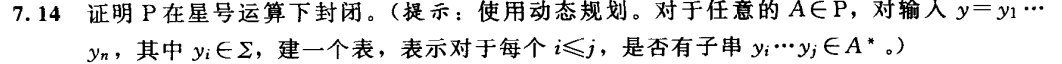
\includegraphics[width=\textwidth]{chapters/imgs/hw_7_14.png}
  \caption{}
  \label{fig:hw_7_14}
\end{figure}

\subsubsection*{证明}

我们证明：若 $A \in \mathbf{P}$，则 $A^* \in \mathbf{P}$。

设 $A \in \mathbf{P}$，则存在一个确定性多项式时间判定机 $M_A$，对任意长度为 $m$ 的输入，都能在时间 $O(m^c)$ 内判定其是否属于 $A$，其中 $c$ 是某个固定常数。下面构造一个确定性多项式时间算法判定 $A^*$。

\paragraph{关键思路：动态规划.}
设输入字符串为
\[
    y = y_1 y_2 \cdots y_n,
\]
其中每个 $y_i \in \Sigma$。当 $n=0$ 时，$y=\varepsilon$，而 $\varepsilon \in A^*$ 恒成立，因此可直接接受。

对非空输入，我们建立一个布尔表 $T$。对任意 $1 \le i \le j \le n$，定义
\[
    T[i][j] =
    \begin{cases}
        \mathbf{true}, & \text{若子串 } y_i y_{i+1} \cdots y_j \in A^*, \\
        \mathbf{false}, & \text{否则。}
    \end{cases}
\]
最后只需检查 $T[1][n]$ 是否为真。

\paragraph{递推关系.}
子串 $y_i \cdots y_j$ 属于 $A^*$，当且仅当它可以写成
\[
    (y_i \cdots y_{k-1})(y_k \cdots y_j),
\]
其中前半段属于 $A^*$，后半段属于 $A$。这里允许前半段为空串；当 $k=i$ 时，前半段就是 $\varepsilon$，显然属于 $A^*$。

因此，对每个 $i \le j$ 有
\[
    T[i][j]
    =
    \bigvee_{k=i}^{j}
    \Bigl(
        \bigl(k=i \text{ 或 } T[i][k-1]\bigr)
        \wedge
        (y_k \cdots y_j \in A)
    \Bigr).
\]

\subsubsection*{算法构造}

\begin{myalgo}{判定 $A^*$ 的算法 $M^*$}
\begin{algorithmic}[1]
  \Require 输入字符串 $y = y_1 y_2 \cdots y_n$
  \Ensure 若 $y \in A^*$ 则接受，否则拒绝
  \If{$n = 0$}
    \State \textbf{接受}
  \EndIf
  \State 建立一个 $n \times n$ 的布尔表 $T$，初值全为 \textbf{false}
  \For{$\ell = 1$ \textbf{to} $n$}
    \For{$i = 1$ \textbf{to} $n-\ell+1$}
      \State $j \gets i+\ell-1$
      \For{$k = i$ \textbf{to} $j$}
        \If{$k=i$}
          \State $left \gets \mathbf{true}$
        \Else
          \State $left \gets T[i][k-1]$
        \EndIf
        \If{$left = \mathbf{true}$ \textbf{and} $M_A$ 接受子串 $y_k \cdots y_j$}
          \State $T[i][j] \gets \mathbf{true}$
          \State \textbf{break}
        \EndIf
      \EndFor
    \EndFor
  \EndFor
  \If{$T[1][n] = \mathbf{true}$}
    \State \textbf{接受}
  \Else
    \State \textbf{拒绝}
  \EndIf
\end{algorithmic}
\end{myalgo}

\subsubsection*{正确性证明}

对长度 $\ell = j-i+1$ 做归纳，证明算法算出的每个 $T[i][j]$ 都正确刻画了子串 $y_i \cdots y_j$ 是否属于 $A^*$。

\paragraph{基础情形：$\ell=1$.}
此时子串只有一个字符 $y_i$。算法会检查唯一的分割点 $k=i$，此时前半段为空串，自动视为属于 $A^*$；因此
\[
    T[i][i] = \mathbf{true}
    \iff
    M_A \text{ 接受 } y_i
    \iff
    y_i \in A.
\]
而长度为 $1$ 的字符串属于 $A^*$，只能是它本身就属于 $A$，故此时结论成立。

\paragraph{归纳步骤：$\ell \ge 2$.}
假设所有长度小于 $\ell$ 的子串对应的表项都已被正确计算。考虑任意长度为 $\ell$ 的子串 $y_i \cdots y_j$。

根据算法，$T[i][j]$ 被置为 \textbf{true} 当且仅当存在某个 $k \in [i,j]$，使得
\[
    \bigl(k=i \text{ 或 } T[i][k-1]=\mathbf{true}\bigr)
    \quad \text{且} \quad
    M_A \text{ 接受 } y_k \cdots y_j.
\]
由归纳假设可知，当 $k>i$ 时，$T[i][k-1]=\mathbf{true}$ 等价于 $y_i \cdots y_{k-1} \in A^*$；而当 $k=i$ 时，前半段为空串 $\varepsilon \in A^*$。同时，$M_A$ 的正确性保证
\[
    M_A \text{ 接受 } y_k \cdots y_j
    \iff
    y_k \cdots y_j \in A.
\]
于是，
\[
    T[i][j]=\mathbf{true}
    \iff
    \text{存在某个分割点 } k,\ 
    y_i \cdots y_{k-1} \in A^*
    \text{ 且 }
    y_k \cdots y_j \in A.
\]
这正是 $y_i \cdots y_j \in A^*$ 的定义。因此长度为 $\ell$ 的情形也成立。

由归纳法，所有表项都正确，特别地，
\[
    T[1][n] = \mathbf{true}
    \iff
    y \in A^*.
\]
因此算法 $M^*$ 正确判定 $A^*$。

\subsubsection*{时间复杂度分析}

\begin{itemize}
  \item 表 $T$ 一共有 $O(n^2)$ 个表项。
  \item 对每个表项 $T[i][j]$，算法至多枚举 $n$ 个分割点 $k$。
  \item 对每个 $k$，至多调用一次 $M_A$ 判定子串 $y_k \cdots y_j$；该子串长度不超过 $n$，因此耗时为 $O(n^c)$。
\end{itemize}

故总时间复杂度为
\[
    O(n^2) \cdot O(n) \cdot O(n^c) = O(n^{c+3}),
\]
这是关于输入长度 $n$ 的多项式时间。

因此，$M^*$ 是一个确定性多项式时间判定算法，从而
\[
    A^* \in \mathbf{P}.
\]
由于 $A \in \mathbf{P}$ 是任意的，得到
\[
    A \in \mathbf{P} \implies A^* \in \mathbf{P}.
\]
故 $\mathbf{P}$ 在星号运算下封闭。

\paragraph{案：} 用动态规划记录每个子串是否已经能被分解成若干个属于 $A$ 的片段；这样避免了对所有切分方式做指数级回溯，从而保持了多项式时间。

\subsection*{7.17}

\begin{figure}[H]
  \centering
  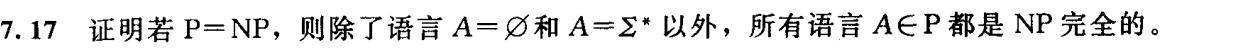
\includegraphics[width=\textwidth]{chapters/imgs/hw_7_17.png}
  \caption{}
  \label{fig:hw_7_17}
\end{figure}

\begin{proof}
采用多项式时间 many-one 归约作为 NP 完全性的定义。假设
\[
P=NP.
\]
任取语言 $A\in P$，且
\[
A\neq \varnothing,\qquad A\neq \Sigma^*.
\]
由于 $A\in P\subseteq NP$，故有
\[
A\in NP.
\]

下面证明 $A$ 是 NP-hard 的。任取 $L\in NP$。由假设 $P=NP$，可得
\[
L\in P.
\]
因此存在一个多项式时间算法可以判定 $L$。

又因为 $A\neq\varnothing$，所以存在字符串 $y_1\in A$；因为
$A\neq\Sigma^*$，所以存在字符串 $y_0\notin A$。定义函数
$f:\Sigma^*\to\Sigma^*$ 为
\[
f(x)=
\begin{cases}
y_1, & x\in L,\\
y_0, & x\notin L.
\end{cases}
\]
由于 $L\in P$，可以在多项式时间内判断 $x\in L$ 是否成立；
而 $y_0,y_1$ 是固定字符串，因此 $f$ 是多项式时间可计算函数。

对任意 $x\in\Sigma^*$，若 $x\in L$，则
\[
f(x)=y_1\in A;
\]
若 $x\notin L$，则
\[
f(x)=y_0\notin A.
\]
因此
\[
x\in L \iff f(x)\in A.
\]
所以
\[
L\leq_p A.
\]
由于 $L\in NP$ 是任意的，故
\[
\forall L\in NP,\quad L\leq_p A.
\]
因此 $A$ 是 NP-hard 的。

综上，$A\in NP$ 且 $A$ 是 NP-hard，所以 $A$ 是 NP 完全的。
\end{proof}

\paragraph{案：} 这道题最值得玩味的地方在于，规约并不只是“把一个难题机械地变成另一个难题”，而是在不同问题的表述之间传递同一个判定结构。平时我们把多项式时间规约理解为“把未知问题压到一个已知的标准问题上”；而在假设 $P=NP$ 之后，原本“难”与“易”的边界被彻底抹平了。于是，任何一个既不是空集、也不是全集的语言 $A\in P$，都可以作为这种传递的落点。证明里只需固定一个属于 $A$ 的字符串 $y_1$ 和一个不属于 $A$ 的字符串 $y_0$，就能把任意 $L\in NP$ 的真假判定压缩成对 $A$ 的真假判定。换句话说，从一个问题到另一个问题的规约，可以理解成是在不断切换看问题的视角；而当这些视角被压缩到极致时，最后剩下的其实只是最基本的“是或否”的数学判定。

\subsection*{7.23}

\begin{figure}[H]
  \centering
  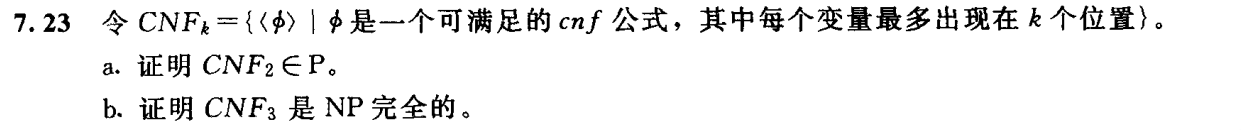
\includegraphics[width=\textwidth]{chapters/imgs/hw_7_23.png}
  \caption{}
  \label{fig:hw_7_23}
\end{figure}

\[
CNF_k=\{\langle \phi\rangle \mid \phi \text{ 是可满足的 CNF 公式，且每个变量至多出现 }k\text{ 次}\}.
\]

\paragraph{(a) 证明 \(CNF_2\in P\).}

设输入是一个 CNF 公式 $\phi$，并且其中每个变量在整个公式中出现的总次数至多为 $2$。记输入长度为 $N$，这里 $N$ 可以取为 $\phi$ 中文字出现的总数。

我们构造如下确定性算法，用来判定在每个变量至多出现两次的前提下，CNF 公式 $\phi$ 是否可满足。

\begin{myalgo}{判定 $2$-出现 CNF 公式 $\phi$ 是否可满足的算法}
\begin{algorithmic}[1]
  \Require 一个 CNF 公式 $\phi$，其中每个变量至多出现 $2$ 次
  \Ensure 若 $\phi$ 可满足则接受，否则拒绝
  \State $\psi \gets \phi$
  \While{$\psi$ 中仍含有变量}
    \If{$\psi$ 中存在空子句}
      \State \textbf{拒绝}
    \EndIf
    \State 任取一个仍在 $\psi$ 中出现的变量 $x$
    \If{$x$ 在 $\psi$ 中只正出现，或只负出现}
      \State 令 $x$ 取使这些子句满足的真值
      \State 从 $\psi$ 中删除所有包含 $x$ 或 $\neg x$ 的子句
    \Else
      \State $x$ 在 $\psi$ 中恰好一次正出现、一次负出现
      \State 设这两个子句分别为 $C_1=(x \vee A)$ 和 $C_2=(\neg x \vee B)$
      \State 从 $\psi$ 中删除 $C_1$ 和 $C_2$
      \State 构造归结子句 $D=A \vee B$
      \State 在 $D$ 中删去重复文字
      \If{$D$ 同时含有某个变量 $y$ 与 $\neg y$}
        \State 丢弃 $D$ \Comment{$D$ 为重言式}
      \ElsIf{$D$ 为空子句}
        \State \textbf{拒绝}
      \Else
        \State 将 $D$ 加入 $\psi$
      \EndIf
    \EndIf
  \EndWhile
  \If{$\psi$ 中存在空子句}
    \State \textbf{拒绝}
  \Else
    \State \textbf{接受}
  \EndIf
\end{algorithmic}
\end{myalgo}

\paragraph{算法保持的性质.}
在算法执行过程中，始终保持“每个变量至多出现两次”这一性质。

\begin{itemize}
  \item 在第一种操作中，我们只是删除一些子句，因此每个变量的出现次数只会减少。
  \item 在第二种操作中，被消去的变量 $x$ 被完全删除。对于其他变量，它们在新子句 $D$ 中的出现，仅仅来自原来 $A$ 或 $B$ 中的出现，因此它们的总出现次数不会增加。
\end{itemize}

因此每次循环中，对被选中的变量 $x$，确实只会落入算法中的两种情形之一。

\paragraph{正确性证明.}
我们证明：每次循环对公式做的变换都保持可满足性。

\paragraph{第一种情形：$x$ 只以同一种极性出现.}
不妨设 $x$ 只正出现。令
\[
\psi = C_1 \wedge C_2 \wedge \cdots \wedge C_t \wedge R,
\]
其中 $C_1,\dots,C_t$ 是所有含有 $x$ 的子句，$R$ 中不含 $x$。

设 $\psi'$ 为从 $\psi$ 中删除 $C_1,\dots,C_t$ 后得到的公式，也就是算法更新后的公式。

\begin{itemize}
  \item 若 $\psi$ 可满足，则取一个满足赋值。把其中 $x$ 的取值改成 $1$ 后，所有 $C_i$ 仍然满足，而 $R$ 不受影响。因此该赋值在删去 $C_1,\dots,C_t$ 后仍满足 $\psi'$。
  \item 若 $\psi'$ 可满足，则把满足 $\psi'$ 的赋值扩张为 $x=1$，即可满足所有 $C_i$，从而满足 $\psi$。
\end{itemize}

故 $\psi$ 可满足当且仅当 $\psi'$ 可满足。若 $x$ 只负出现，证明完全类似。

\paragraph{第二种情形：$x$ 一正一负各出现一次.}
设
\[
\psi = (x \vee A)\wedge (\neg x \vee B)\wedge R,
\]
其中 $A,B,R$ 都不含变量 $x$。算法将其替换为
\[
\psi' = (A \vee B)\wedge R,
\]
若 $A \vee B$ 是重言式则直接删除该子句；若 $A \vee B$ 为空子句则立即拒绝。

下面证明 $\psi$ 与 $\psi'$ 等可满足。

\begin{itemize}
  \item 若 $\psi$ 可满足，取其在除 $x$ 之外各变量上的限制赋值。由于
  \[
  (x \vee A)\wedge (\neg x \vee B)
  \]
  被满足，因此若 $x=0$ 则必须有 $A=1$，若 $x=1$ 则必须有 $B=1$。无论哪种情况，都有 $A \vee B = 1$，故该限制赋值满足 $\psi'$。
  \item 若 $\psi'$ 可满足，则在满足 $\psi'$ 的赋值下，$A \vee B = 1$。若 $A=1$，令 $x=0$，则 $(\neg x \vee B)$ 自动为真，且 $(x \vee A)$ 也为真；若 $A=0$，则必有 $B=1$，令 $x=1$ 即可。于是该赋值可扩张为 $\psi$ 的满足赋值。
\end{itemize}

故 $\psi$ 可满足当且仅当 $\psi'$ 可满足。

由以上两种情形可知，算法每一步都保持可满足性不变。最终若算法拒绝，则一定是产生了空子句，而空子句不可满足；若算法接受，则所有变量都已被消去且未出现空子句，此时剩余公式为空合取，必可满足。因此算法正确。

\paragraph{时间复杂度分析.}
令 $N$ 为输入公式中出现的文字总数。

\begin{itemize}
  \item 每次循环至少消去一个变量。
  \item 更重要的是，每次循环都会使当前公式中的文字总数严格下降。
  \item 在第一种情形中，至少删除一个包含 $x$ 的文字。
  \item 在第二种情形中，原来的两个子句一共含有
  \[
  |A| + |B| + 2
  \]
  个文字，而加入的新子句最多只含有
  \[
  |A| + |B|
  \]
  个文字，因此文字总数至少减少 $2$。
\end{itemize}

所以循环次数至多为 $N$ 次。若采用朴素实现，每次循环中扫描当前公式、定位相关子句并构造归结子句，时间均为 $O(N)$。因此总时间复杂度为
\[
O(N^2),
\]
是多项式时间。

故
\[
CNF_2 \in P.
\]

\paragraph{(b) 证明 \(CNF_3\) 是 NP 完全的。}

\paragraph{第一步：证明 \(CNF_3\in NP\).}
给定一个真值赋值，我们可以在多项式时间内逐个检查所有子句是否被满足，并统计每个变量在公式中的出现次数是否至多为 $3$。因此
\[
CNF_3 \in NP.
\]

\paragraph{第二步：证明 \(CNF_3\) 是 NP-hard.}
我们从标准的
\[
\textsc{CNF-SAT}
=
\{\langle \phi \rangle \mid \phi \text{ 是可满足的 CNF 公式}\}
\]
做多项式时间 many-one 归约。

设 $\phi$ 是任意一个 CNF 公式。对 $\phi$ 中每个变量 $x$，记它在 $\phi$ 中总共出现 $d_x$ 次。

\begin{itemize}
  \item 若 $d_x \le 3$，则保持变量 $x$ 不变。
  \item 若 $d_x > 3$，则把这 $d_x$ 次出现分别替换为新的变量
  \[
  x_1,x_2,\dots,x_{d_x}.
  \]
  若原来第 $i$ 次出现是正文字 $x$，则替换为 $x_i$；若原来第 $i$ 次出现是否定文字 $\neg x$，则替换为 $\neg x_i$。
\end{itemize}

为了强制这些新变量取相同真值，对每个满足 $d_x>3$ 的原变量 $x$ 再加入如下 $d_x$ 个子句：
\[
(\neg x_1 \vee x_2)\wedge
(\neg x_2 \vee x_3)\wedge \cdots \wedge
(\neg x_{d_x-1} \vee x_{d_x})\wedge
(\neg x_{d_x} \vee x_1).
\]

把经过上述替换后的原子句，与所有新加入的环形子句合起来，得到新公式 $\psi$。这就是归约输出。

\paragraph{归约的大小与出现次数控制.}
对每个被拆开的变量 $x$：

\begin{itemize}
  \item 每个新变量 $x_i$ 在替换后的原公式部分中恰好出现一次。
  \item 在环形子句中，$x_i$ 恰好正出现一次、负出现一次。
\end{itemize}

因此每个 $x_i$ 在 $\psi$ 中总共恰好出现 $3$ 次；而未被拆开的变量本来就至多出现 $3$ 次。因此 $\psi$ 中每个变量至多出现 $3$ 次，即
\[
\psi \text{ 的确满足 } CNF_3 \text{ 定义中的出现次数限制。}
\]

同时，若 $\phi$ 的总文字数为 $N$，则新引入的变量数和子句数都只是 $O(N)$，故整个构造可在多项式时间内完成。

\paragraph{正确性：若 \(\phi\) 可满足，则 \(\psi\) 可满足.}
设 $\alpha$ 是 $\phi$ 的一个满足赋值。

\begin{itemize}
  \item 对于未拆开的变量 $x$，令其在 $\psi$ 中保持同样取值。
  \item 对于被拆开的变量 $x$，令
  \[
  x_1=x_2=\cdots=x_{d_x}=\alpha(x).
  \]
\end{itemize}

这样，替换后的每个原子句都仍然满足，因为我们只是把原来某一次出现的 $x$ 或 $\neg x$ 换成了与 $\alpha(x)$ 同值的新变量。另一方面，每个环形子句
\[
(\neg x_i \vee x_{i+1})
\]
在上述赋值下都变成
\[
(\neg \alpha(x) \vee \alpha(x)),
\]
恒为真。因此 $\psi$ 可满足。

\paragraph{正确性：若 \(\psi\) 可满足，则 \(\phi\) 可满足.}
设 $\beta$ 是 $\psi$ 的一个满足赋值。我们证明：对每个被拆开的原变量 $x$，一定有
\[
\beta(x_1)=\beta(x_2)=\cdots=\beta(x_{d_x}).
\]

若不然，则在循环序列
\[
x_1,x_2,\dots,x_{d_x},x_1
\]
中，必存在某个相邻位置满足
\[
\beta(x_i)=1,\qquad \beta(x_{i+1})=0,
\]
其中下标按模 $d_x$ 计算。于是子句
\[
(\neg x_i \vee x_{i+1})
\]
在 $\beta$ 下取值为假，这与 $\beta$ 满足 $\psi$ 矛盾。故所有 $x_i$ 必同值。

现在定义原公式 $\phi$ 的赋值 $\alpha$：

\begin{itemize}
  \item 对未拆开的变量 $x$，令 $\alpha(x)=\beta(x)$。
  \item 对被拆开的变量 $x$，令 $\alpha(x)=\beta(x_1)$。
\end{itemize}

由于同一个原变量 $x$ 的所有副本 $x_i$ 在 $\beta$ 下同值，故 $\phi$ 中每个原子句在 $\alpha$ 下的真假，与 $\psi$ 中对应替换后子句在 $\beta$ 下的真假完全一致。因为后者都被满足，所以前者也都被满足。因此 $\phi$ 可满足。

\paragraph{归约结论.}
我们已经证明
\[
\phi \in \textsc{CNF-SAT}
\iff
\psi \in CNF_3.
\]
因此
\[
\textsc{CNF-SAT} \le_p CNF_3.
\]
由于 $\textsc{CNF-SAT}$ 是 NP 完全的，故 $CNF_3$ 是 NP-hard 的。

综合两步，得到
\[
CNF_3 \in NP
\quad \text{且} \quad
CNF_3 \text{ 是 NP-hard}.
\]
因此
\[
CNF_3 \text{ 是 NP 完全的}.
\]

\subsection*{7.27}

\begin{figure}[h]
  \centering
  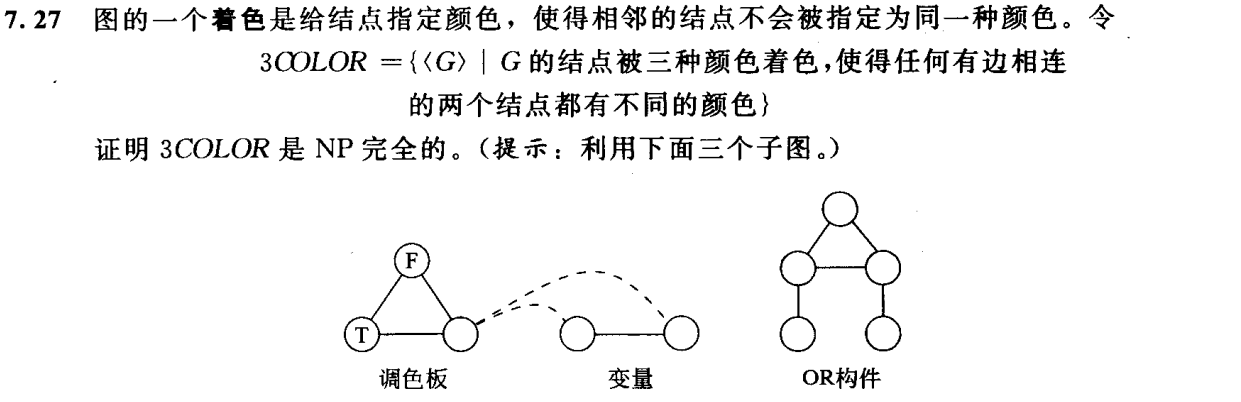
\includegraphics[width=\textwidth]{chapters/imgs/hw_7_27.png}
  \caption{}
  \label{fig:hw_7_27}
\end{figure}



\subsection*{7.28}


\begin{figure}[H]
  \centering
  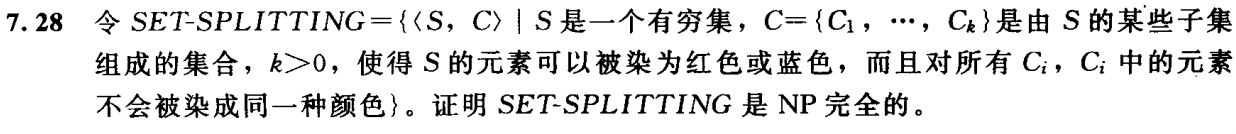
\includegraphics[width=\textwidth]{chapters/imgs/hw_7_28.png}
  \caption{}
  \label{fig:hw_7_28}
\end{figure}

\subsection*{7.29}

\begin{figure}[H]
  \centering
  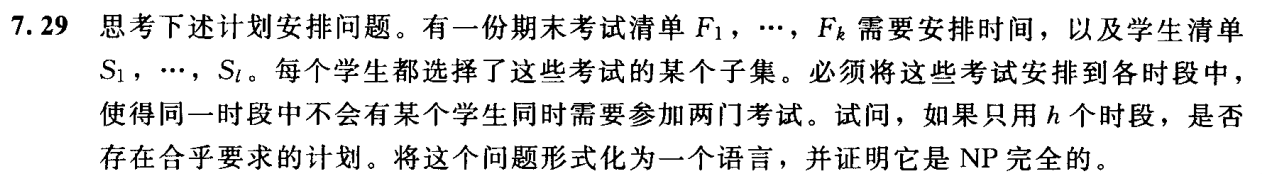
\includegraphics[width=\textwidth]{chapters/imgs/hw_7_29.png}
  \caption{}
  \label{fig:hw_7_29}
\end{figure}

\subsection*{7.30}

\begin{figure}[H]
  \centering
  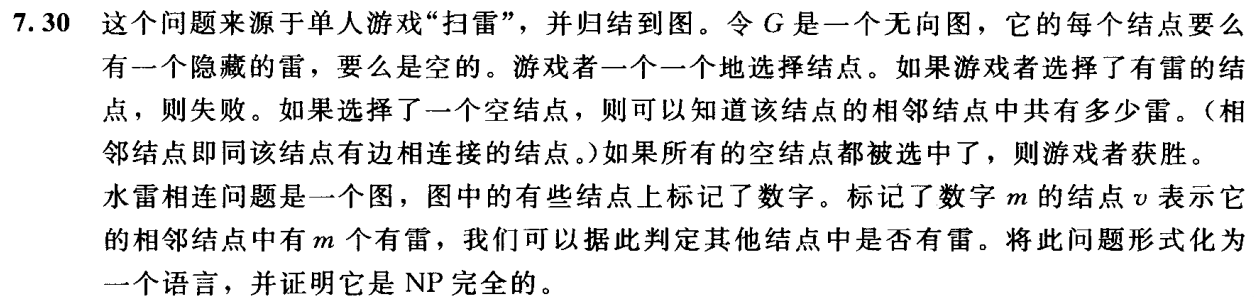
\includegraphics[width=\textwidth]{chapters/imgs/hw_7_30.png}
  \caption{}
  \label{fig:hw_7_30}
\end{figure}

\subsection*{7.32}

\begin{figure}[H]
  \centering
  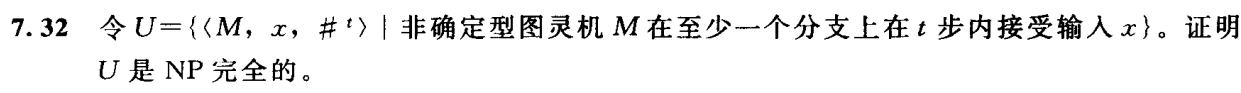
\includegraphics[width=\textwidth]{chapters/imgs/hw_7_32.png}
  \caption{}
  \label{fig:hw_7_32}
\end{figure}

\subsection*{7.34}


\begin{figure}[H]
  \centering
  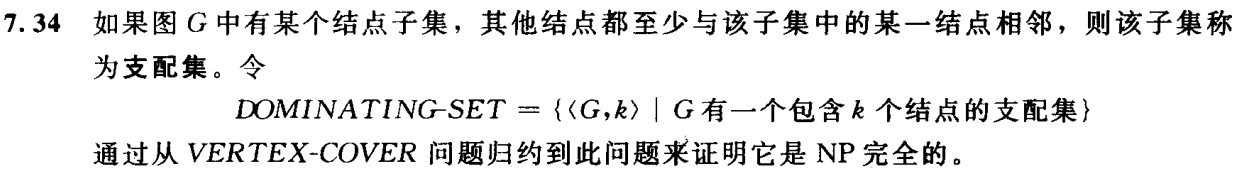
\includegraphics[width=\textwidth]{chapters/imgs/hw_7_34.png}
  \caption{}
  \label{fig:hw_7_34}
\end{figure}

\subsection*{7.36}

\begin{figure}[H]
  \centering
  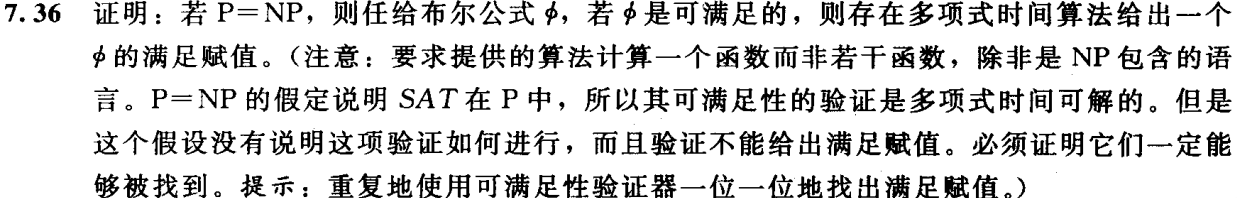
\includegraphics[width=0.8\textwidth]{chapters/imgs/hw_7_36.png}
  \caption{}
  \label{fig:hw_7_36}
\end{figure}

\subsection*{7.39}

\begin{figure}[H]
  \centering
  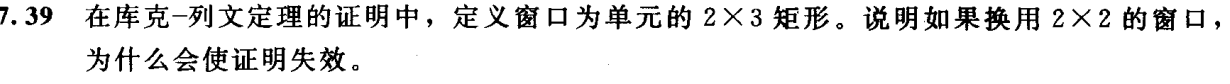
\includegraphics[width=0.8\textwidth]{chapters/imgs/hw_7_39.png}
  \caption{}
  \label{fig:hw_7_39}
\end{figure}

\subsection*{7.40}


\begin{figure}[H]
  \centering
  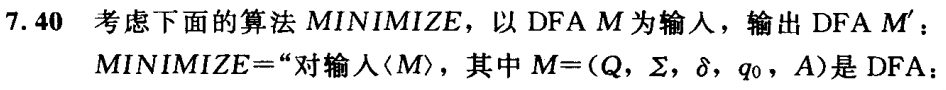
\includegraphics[width=0.8\textwidth]{chapters/imgs/hw_7_40_p1.png}
  \caption{}
  \label{fig:hw_7_40_p1}
\end{figure}

\begin{figure}[H]
  \centering
  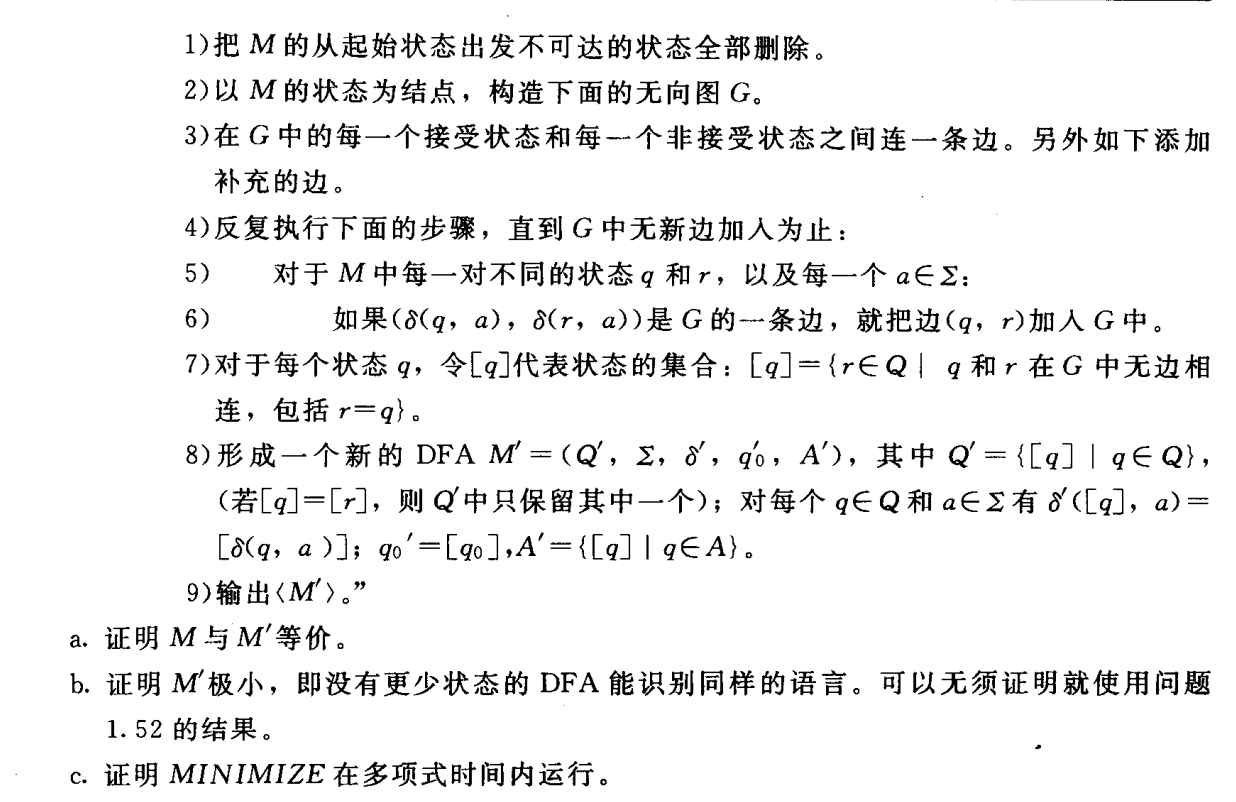
\includegraphics[width=0.8\textwidth]{chapters/imgs/hw_7_40_p2.png}
  \caption{}
  \label{fig:hw_7_40_p2}
\end{figure}

\subsection*{7.42}

\begin{figure}[H]
  \centering
  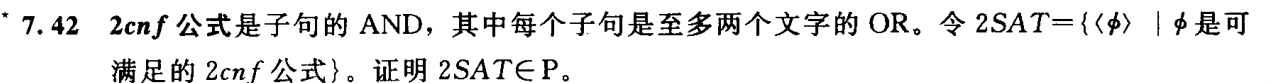
\includegraphics[width=\textwidth]{chapters/imgs/hw_7_42.png}
  \caption{}
  \label{fig:hw_7_42}
\end{figure}

\clearpage
